% Copyright 2004 by Till Tantau <tantau@users.sourceforge.net>.
%
% In principle, this file can be redistributed and/or modified under
% the terms of the GNU Public License, version 2.
%
% However, this file is supposed to be a template to be modified
% for your own needs. For this reason, if you use this file as a
% template and not specifically distribute it as part of a another
% package/program, I grant the extra permission to freely copy and
% modify this file as you see fit and even to delete this copyright
% notice. 

\documentclass{beamer}

% There are many different themes available for Beamer. A comprehensive
% list with examples is given here:
% http://deic.uab.es/~iblanes/beamer_gallery/index_by_theme.html
% You can uncomment the themes below if you would like to use a different
% one:
%\usetheme{AnnArbor}
%\usetheme{Antibes}
%\usetheme{Bergen}
%\usetheme{Berkeley}
%\usetheme{Berlin}
%\usetheme{Boadilla}
%\usetheme{boxes}
%\usetheme{CambridgeUS}
%\usetheme{Copenhagen}
%\usetheme{Darmstadt}
%\usetheme{default}
%\usetheme{Frankfurt}
%\usetheme{Goettingen}
%\usetheme{Hannover}
%\usetheme{Ilmenau}
%\usetheme{JuanLesPins}
%\usetheme{Luebeck}
\usetheme{Madrid}
%\usetheme{Malmoe}
%\usetheme{Marburg}
%\usetheme{Montpellier}
%\usetheme{PaloAlto}
%\usetheme{Pittsburgh}
%\usetheme{Rochester}
%\usetheme{Singapore}
%\usetheme{Szeged}
%\usetheme{Warsaw}

\usepackage[utf8]{inputenc} 
\usepackage[T1]{fontenc}
\usepackage{setspace}

\usepackage{listings}
\usepackage{color}

\title[Posterior Regularization]{Prior Knowledge Integration for Neural Machine Translation using Posterior Regularization}

\author{Andrew Drozdov}

% Let's get started
\begin{document}

% Title
\begin{frame}
  \titlepage
\end{frame}
%

% SLIDE
\begin{frame}{Background}{}
\begin{itemize}
\item Neural Machine Translation
\item Posterior Regularization
\end{itemize}
\end{frame}
% SLIDE

% SLIDE
\begin{frame}{Background: Neural Machine Translation}{}
\begin{itemize}
\item Standard Seq2seq.

\begin{align*}
\mathcal{L}(\theta) = \Sigma_n \log P(y^n|x^n;\theta)
\end{align*}

\item It's difficult to incorporate linguistic prior knowledge in discrete symbolic forms (like phrase tables).
\begin{itemize}
\item There are other ways to incorporate linguistic priors. \footnote[frame]{Eriguchi et al. 2017 Learning to Parse and Translate Improves Neural Machine Translation}
\end{itemize}

% https://arxiv.org/pdf/1601.04811.pdf
% Every phrase should be covered in alignment.
\item Example of prior knowledge: coverage constraint.

\item Existing approaches are not scalable.
\begin{itemize}
\item Only works for simple constraints.
\item Not flexible.
\end{itemize}
\end{itemize}

\end{frame}
% SLIDE

% SLIDE
\begin{frame}{Background: Posterior Regularization}{}
\begin{itemize}
\item Posterior regularized likelihood:

\begin{align*}
F(\theta, q) &= \lambda_1 \mathcal{L}(\theta) - \lambda_2 \Sigma_n  \min_{q \in \mathcal{Q}} KL \big( q(y) || P(y|x^n; \theta) \big)
\end{align*}

\item $\mathcal{Q}$ is a constrained posterior set.
\begin{itemize}
\item For instance, bijectivity and symmetry in machine translation.
\end{itemize}

\begin{align*}
\mathcal{Q} &= \{ q(y) : \mathbb{E}_q[\phi(x, y)] \leq b\}
\end{align*}

\item Can be optimized using a simple EM scheme.

\vspace{4mm}
\centering
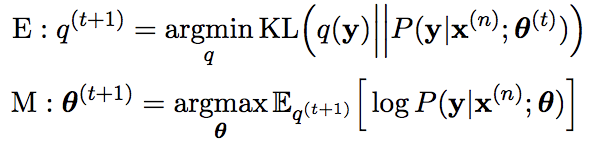
\includegraphics[width=0.75\textheight]{em}

\end{itemize}

\end{frame}
% SLIDE

% SLIDE
\begin{frame}{Model}{}
\begin{itemize}
\item Use a log-linear model rather than a constrained posterior set.

\begin{align*}
\mathcal{J}(\theta, \gamma) &= \lambda_1 \mathcal{L}(\theta) - \lambda_2 \Sigma_n KL \big( Q(y|x^n; \gamma) || P(y|x^n; \theta) \big) \\
Q(y|x^n; \gamma) &= \frac{\exp(\gamma \cdot \phi(x,y))}{\Sigma_{y'} \exp(\gamma \cdot \phi(x,y')}
\end{align*}

% \item $\gamma$ is like inverse temperature. Higher values are more peaked.

\end{itemize}

\end{frame}
% SLIDE

% SLIDE
\begin{frame}{Feature Design}{}
\begin{itemize}
\item Bilingual Dictionary $\phi \in \{0, 1\}$
\item Phrase Table $\phi \in \{0, 1\}$

\item Coverage Constraint $\phi_{CP}(x,y) = \Sigma_{i \in |x|} \log \big( \min (1.0, \Sigma_{j \in |y|} a_{i,j}) \big)$
\begin{itemize}
\item Dependent on sentence lengths.
\end{itemize}

\item Length Ratio $\phi_{LR}(x, y) = \frac{\beta|x|}{|y|}$ if $\beta|x| < |y|$ otherwise $\frac{|y|}{\beta|x|}$

\end{itemize}

\end{frame}
% SLIDE

% SLIDE
\begin{frame}{Training and Inference}{}
\begin{itemize}
\item During training, subsample predicted target sentences.
\begin{center}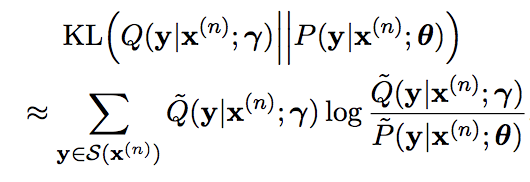
\includegraphics[width=0.5\textheight]{subsample}
\end{center}

\item Normalize the sampled subspace.
\begin{center}
\begin{minipage}{.4\textwidth}
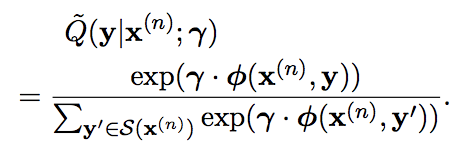
\includegraphics[width=0.5\textheight]{subsampleq}
\end{minipage}
\begin{minipage}{.4\textwidth}
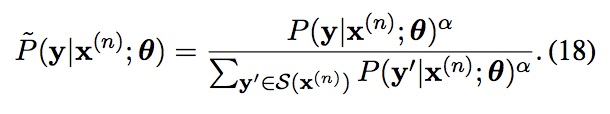
\includegraphics[width=0.5\textheight]{sharpness}
\end{minipage}
\end{center}

\item During inference, generate a candidate list using maximum likelihood only, then rerank by incorporating prior knowledge.

\begin{align*}
\hat{y} &= arg\max_{y \in \mathcal{C}(x)} \{ \log P(y|x;\theta) + \gamma \cdot \phi(x, y) \}
\end{align*}

\end{itemize}

\end{frame}
% SLIDE

% SLIDE
\begin{frame}{Experimental Setup}{}
\begin{itemize}
\item English-to-Chinese Translation.
\item Train RNNSearch for 300k iterations (4 days). Train model of this work (3 days).

\item RNNSearch
\begin{itemize}
\item Word Embedding: 620
\item Hidden Layer: 1000
\item Batch Size: 80
\item AdaDelta
\item Beam Size of 10 during decoding.
\end{itemize}

\item RNNSearch+ThisWork
\begin{itemize}
\item Batch Size: 1
\item Candidates: 80 and $\alpha=0.2$
\item $\lambda_1 = 8 \times 10^{-5}$, $\lambda_2 = 2.5 \times 10^{-4}$
\end{itemize}

\end{itemize}

\end{frame}
% SLIDE

% SLIDE
\begin{frame}{Results}{}
\centering
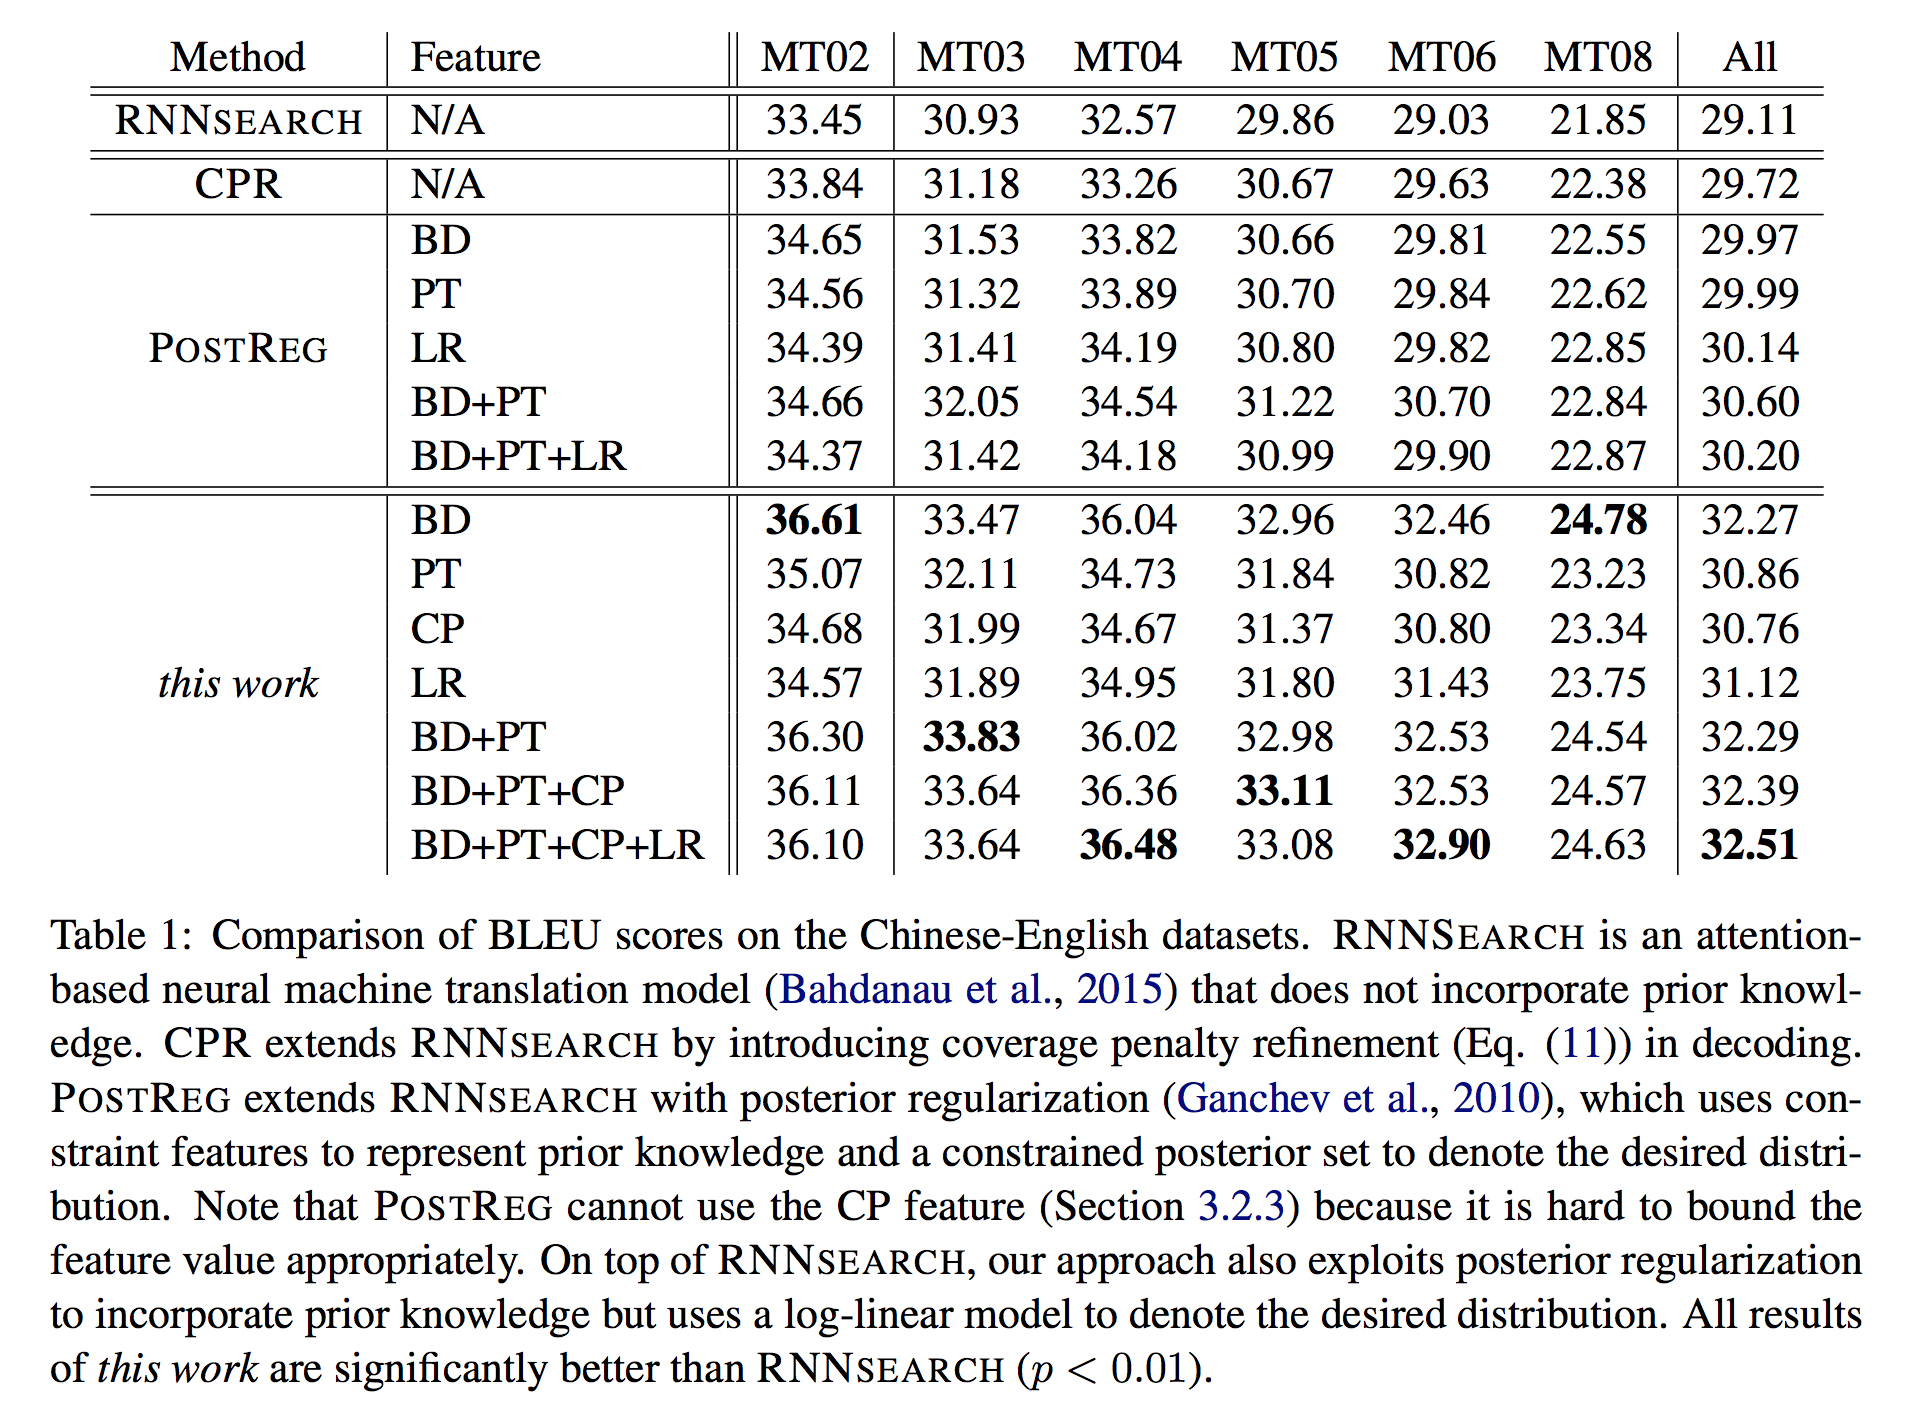
\includegraphics[width=\textheight]{results}
\end{frame}
% SLIDE

% https://arxiv.org/pdf/1606.02003.pdf
% SLIDE
\begin{frame}{Ablation}{}
\centering
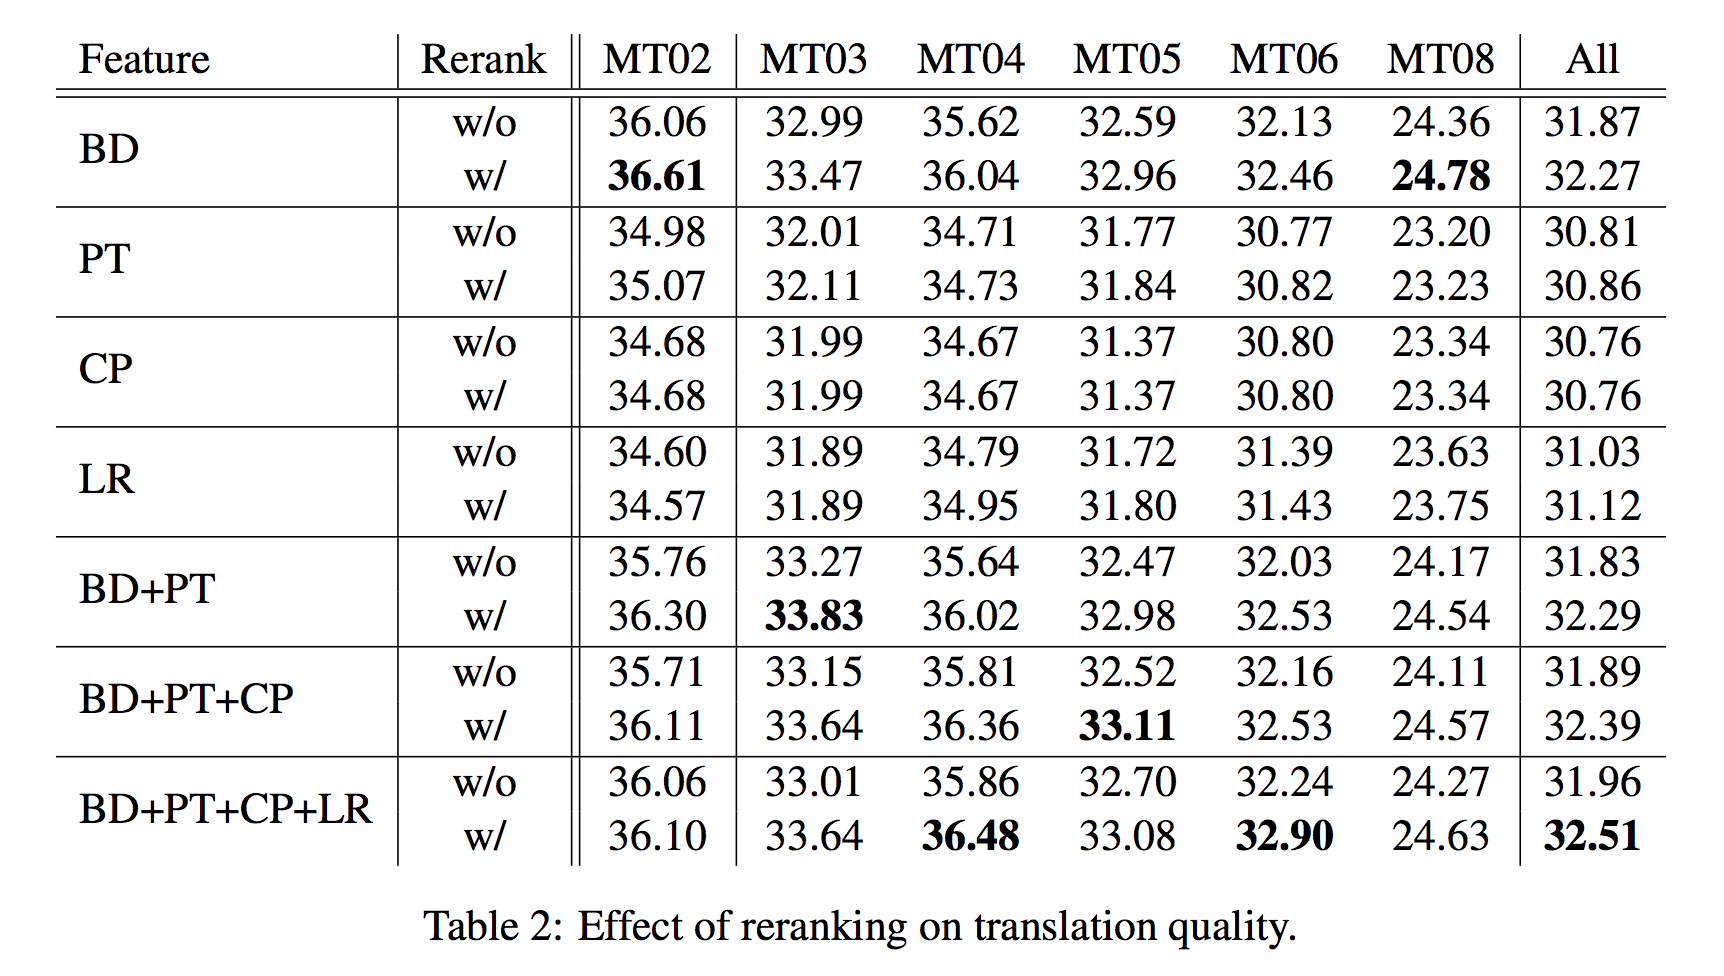
\includegraphics[width=\textheight]{ablation}
\end{frame}
% SLIDE

% SLIDE
\begin{frame}{Examples}{}
\centering
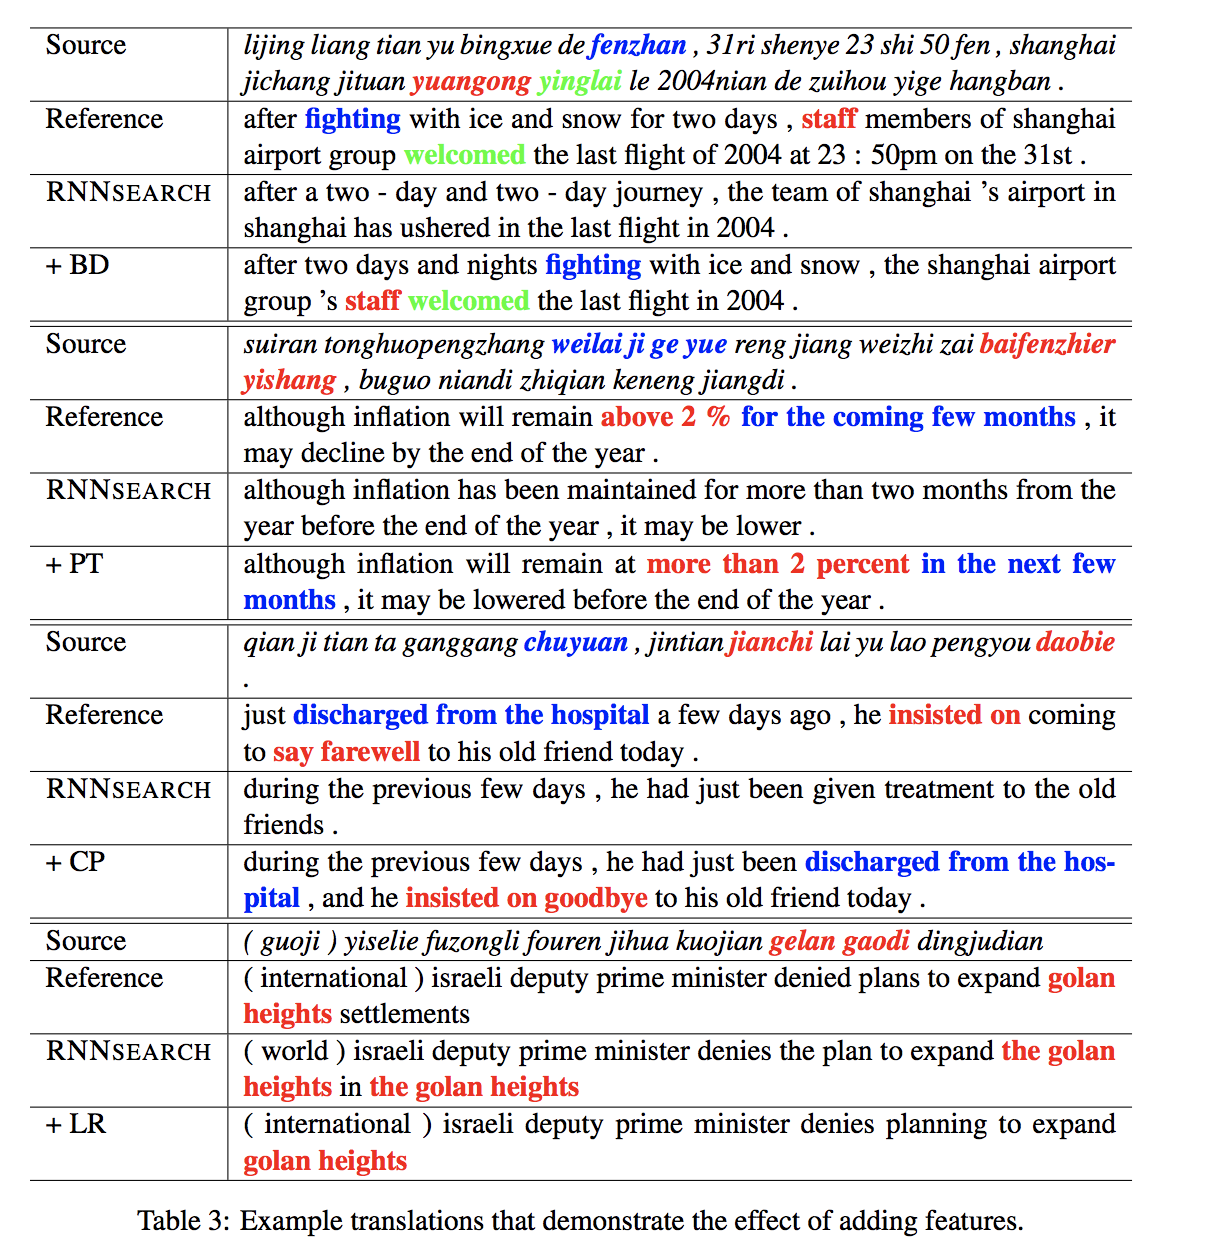
\includegraphics[height=0.8\textheight]{examples}
\end{frame}
% SLIDE


\end{document}


